\section{Elements}\label{sec:element}

The transducer element is the fundamental building block for arrays and the starting point for analysis in Sonar Workbench. For the purpose of generating and analyzing beam patterns, specific electromechanical transduction methods do not need to be modeled; instead, the element's acoustic properties can be captured by modeling vibrations of the element's wetted surface. Hereafter, references to an element's geometry refer to the geometry of the element's wetted surface or face. Sonar Workbench treats each element as a uniformly vibrating surface, which is to say that it only models each surface's fundamental mode of vibration. Analyzing element response requires first, defining the element geometry, and second, evaluating that geometry at a specific acoustic wavelength to produce an element pattern.

\subsection{Element definition}

Sonar Workbench includes support for the element types listed in Table~\ref{tab:ElementTypes}. 

\begin{table}[!ht]
	\begin{center}
		\caption{Included element types}
		\label{tab:ElementTypes}
		\begin{tabular}{c|l} 
			\textbf{Element Type} & \textbf{Type String} \\
			\hline
			Omnidirectional  & \texttt{`OmnidirectionalElement'} \\
			Uniform Line & \texttt{`LinearElement'} \\
			Cosine & \texttt{`CosineElement'} \\
			Circular Piston & \texttt{`CircularPistonElement'} \\
			Rectangular Piston & \texttt{`RectangulerPistonElement'} \\
			Annular Piston & \texttt{`AnnularPistonElement'} \\
			Hexagonal Piston & \texttt{`HexagonalPistonElement'} \\
		\end{tabular}
	\end{center}
\end{table}

An element structure holds the parameters that define the element geometry. The element structure must contain the \texttt{.type} field with a string corresponding to the name of a \texttt{.m} file that generates the corresponding element pattern. Table~\ref{tab:ElementTypes} lists the built-in element type strings, but the user can define additional element types by generating their own element pattern generator script with the same interface. 

The field \texttt{.baffle} dictates whether the element should be baffled by the element frame $y$-$z$ plane (e.g. arrays mounted to platforms) or unbaffled (e.g. towed arrays, sonobuoys). The omnidirectional, uniform line, and cosine elements can all be used with and without baffling. The piston elements' element patterns are all derived from equations assuming the piston is mounted in an infinite rigid baffle; therefore, it is recommended that the user set these element's \texttt{.baffle=1} for best results. Diffraction effects caused by finite baffle dimensions are beyond the scope of Sonar Workbench. 

For visualization purposes, fields \texttt{.shapex}, \texttt{.shapey}, and \texttt{shapez} contain vectors of element shape coordinates. The script \texttt{AddElementShape.m} generates these vectors for the element types listed in Table~\ref{tab:ElementTypes}. The other fields in the element structure depend on the element type, as listed in Table~\ref{tab:ElementFields}.

\begin{table}[!ht]
	\begin{center}
		\caption{Element structure fields}
		\label{tab:ElementFields}
		\begin{tabular}{c|c|l} 
			\textbf{Element Type} & \textbf{Field} & \textbf{Description} \\
			\hline
			\multirow{2}{*}{Uniform Line} & \texttt{.L} & length (m) \\
			& \texttt{.axis} & aligned axis \texttt{`x'}, \texttt{`y'}, \texttt{`z'} \\
			\hline
			Circular Piston & \texttt{.a} & radius (m) \\
			\hline
			\multirow{2}{*}{Rectangular Piston} & \texttt{.w} & width (m) \\
			& \texttt{.h} & height (m) \\
			\hline
			\multirow{2}{*}{Annular Piston} & \texttt{.a} & outer radius (m) \\
			& \texttt{.b} & inner radius (m) \\
			\hline
			Hexagonal Piston & \texttt{.a} & inscribed circle radius (m) \\	
		\end{tabular}
	\end{center}
\end{table}

Listing~\ref{lst:SampleElement} shows the contents of \texttt{SampleElement.m}, which defines a rectangular piston element.

\lstinputlisting[caption={\texttt{SampleElement.m}},label={lst:SampleElement}]{../../examples/SampleElement.m}

The user is free to add additional fields to the element structure for their own purposes. These will be ignored by Sonar Workbench.

\subsection{Element patterns}

Element geometry, coupled with an acoustic wavelength, defines the element pattern. The element pattern is the element's far-field directional response as a function of wavelength, azimuth and elevation, and it can be thought of as a spatial filter. Elements are assumed to be transducers, capable of transmitting and receiving sound, so there is no distinction between transmit and receive element patterns. 

Sonar Workbench uses the acoustic wavelength, $\lambda$, to calculate element patterns because it combines the frequency and sound speed into a single term. It is related to sound speed $c$, frequency $f$ in Hz or $\omega$ in rad/s, and wavenumber $k$ in m$^{-1}$ by
\begin{equation*}
\lambda = \frac{c}{f} = \frac{2\pi{c}}{\omega} = \frac{2\pi}{k}.
\end{equation*}

At its most general, the element pattern is the three-dimensional Fourier transform of the element's complex aperture function, $A(\lambda,x,y,z)$,
\begin{equation}
E(\lambda,\theta,\psi) = \int_{-\infty}^\infty\int_{-\infty}^\infty\int_{-\infty}^\infty A(\lambda,x,y,z)e^{j2\pi\left(\frac{\cos\theta\cos\psi}{\lambda}x + \frac{\cos\theta\sin\psi}{\lambda}y + \frac{\sin\theta}{\lambda}z\right)}dxdydz,\label{eq:VolumetricFT}
\end{equation}
For the piston elements, the element pattern reduces to a two-dimensional Fourier transform, since the element face lies in the $y$-$z$ plane,
\begin{equation}
E_{piston}(\lambda,\theta,\psi) = \int_{-\infty}^\infty\int_{-\infty}^\infty A(\lambda,y,z)e^{j2\pi\left(\frac{\cos\theta\sin\psi}{\lambda}y + \frac{\sin\theta}{\lambda}z\right)}dydz,\label{eq:PlanarFT}
\end{equation}
and for the uniform line array, it further reduces to a one-dimensional Fourier transform,
\begin{equation}
E_{line}(\lambda,\theta,\psi) = \int_{-\infty}^\infty A(\lambda,y)e^{j2\pi\frac{\cos\theta\sin\psi}{\lambda}y}dy,\label{eq:LinearFT}
\end{equation}
for a line array aligned with the $y$ axis. The finite element extents make the integration limits finite. For the simple elements included with Sonar Workbench, the assumption of uniform surface motion means that the aperture function is real-valued and equal to 1 over the entire element surface. This simplifies the integration for certain element geometries. These integrals have analytic solutions, which Sonar Workbench uses instead of evaluating the integrals numerically.

Element patterns are normalized such that they have unity gain along their maximum response axis. \figurename~\ref{fig:ElementPatterns} shows element patterns for each of the included element types listed in Table~\ref{tab:ElementTypes} for a wavelength equal to half of the element's maximum dimension. The uniform line element is aligned with the $y$ axis, and the cosine element is aligned with the $x$ axis. Note that the omnidirectional and cosine element patterns do not depend on wavelength.

\begin{sidewaysfigure}[!ht]
\begin{center}
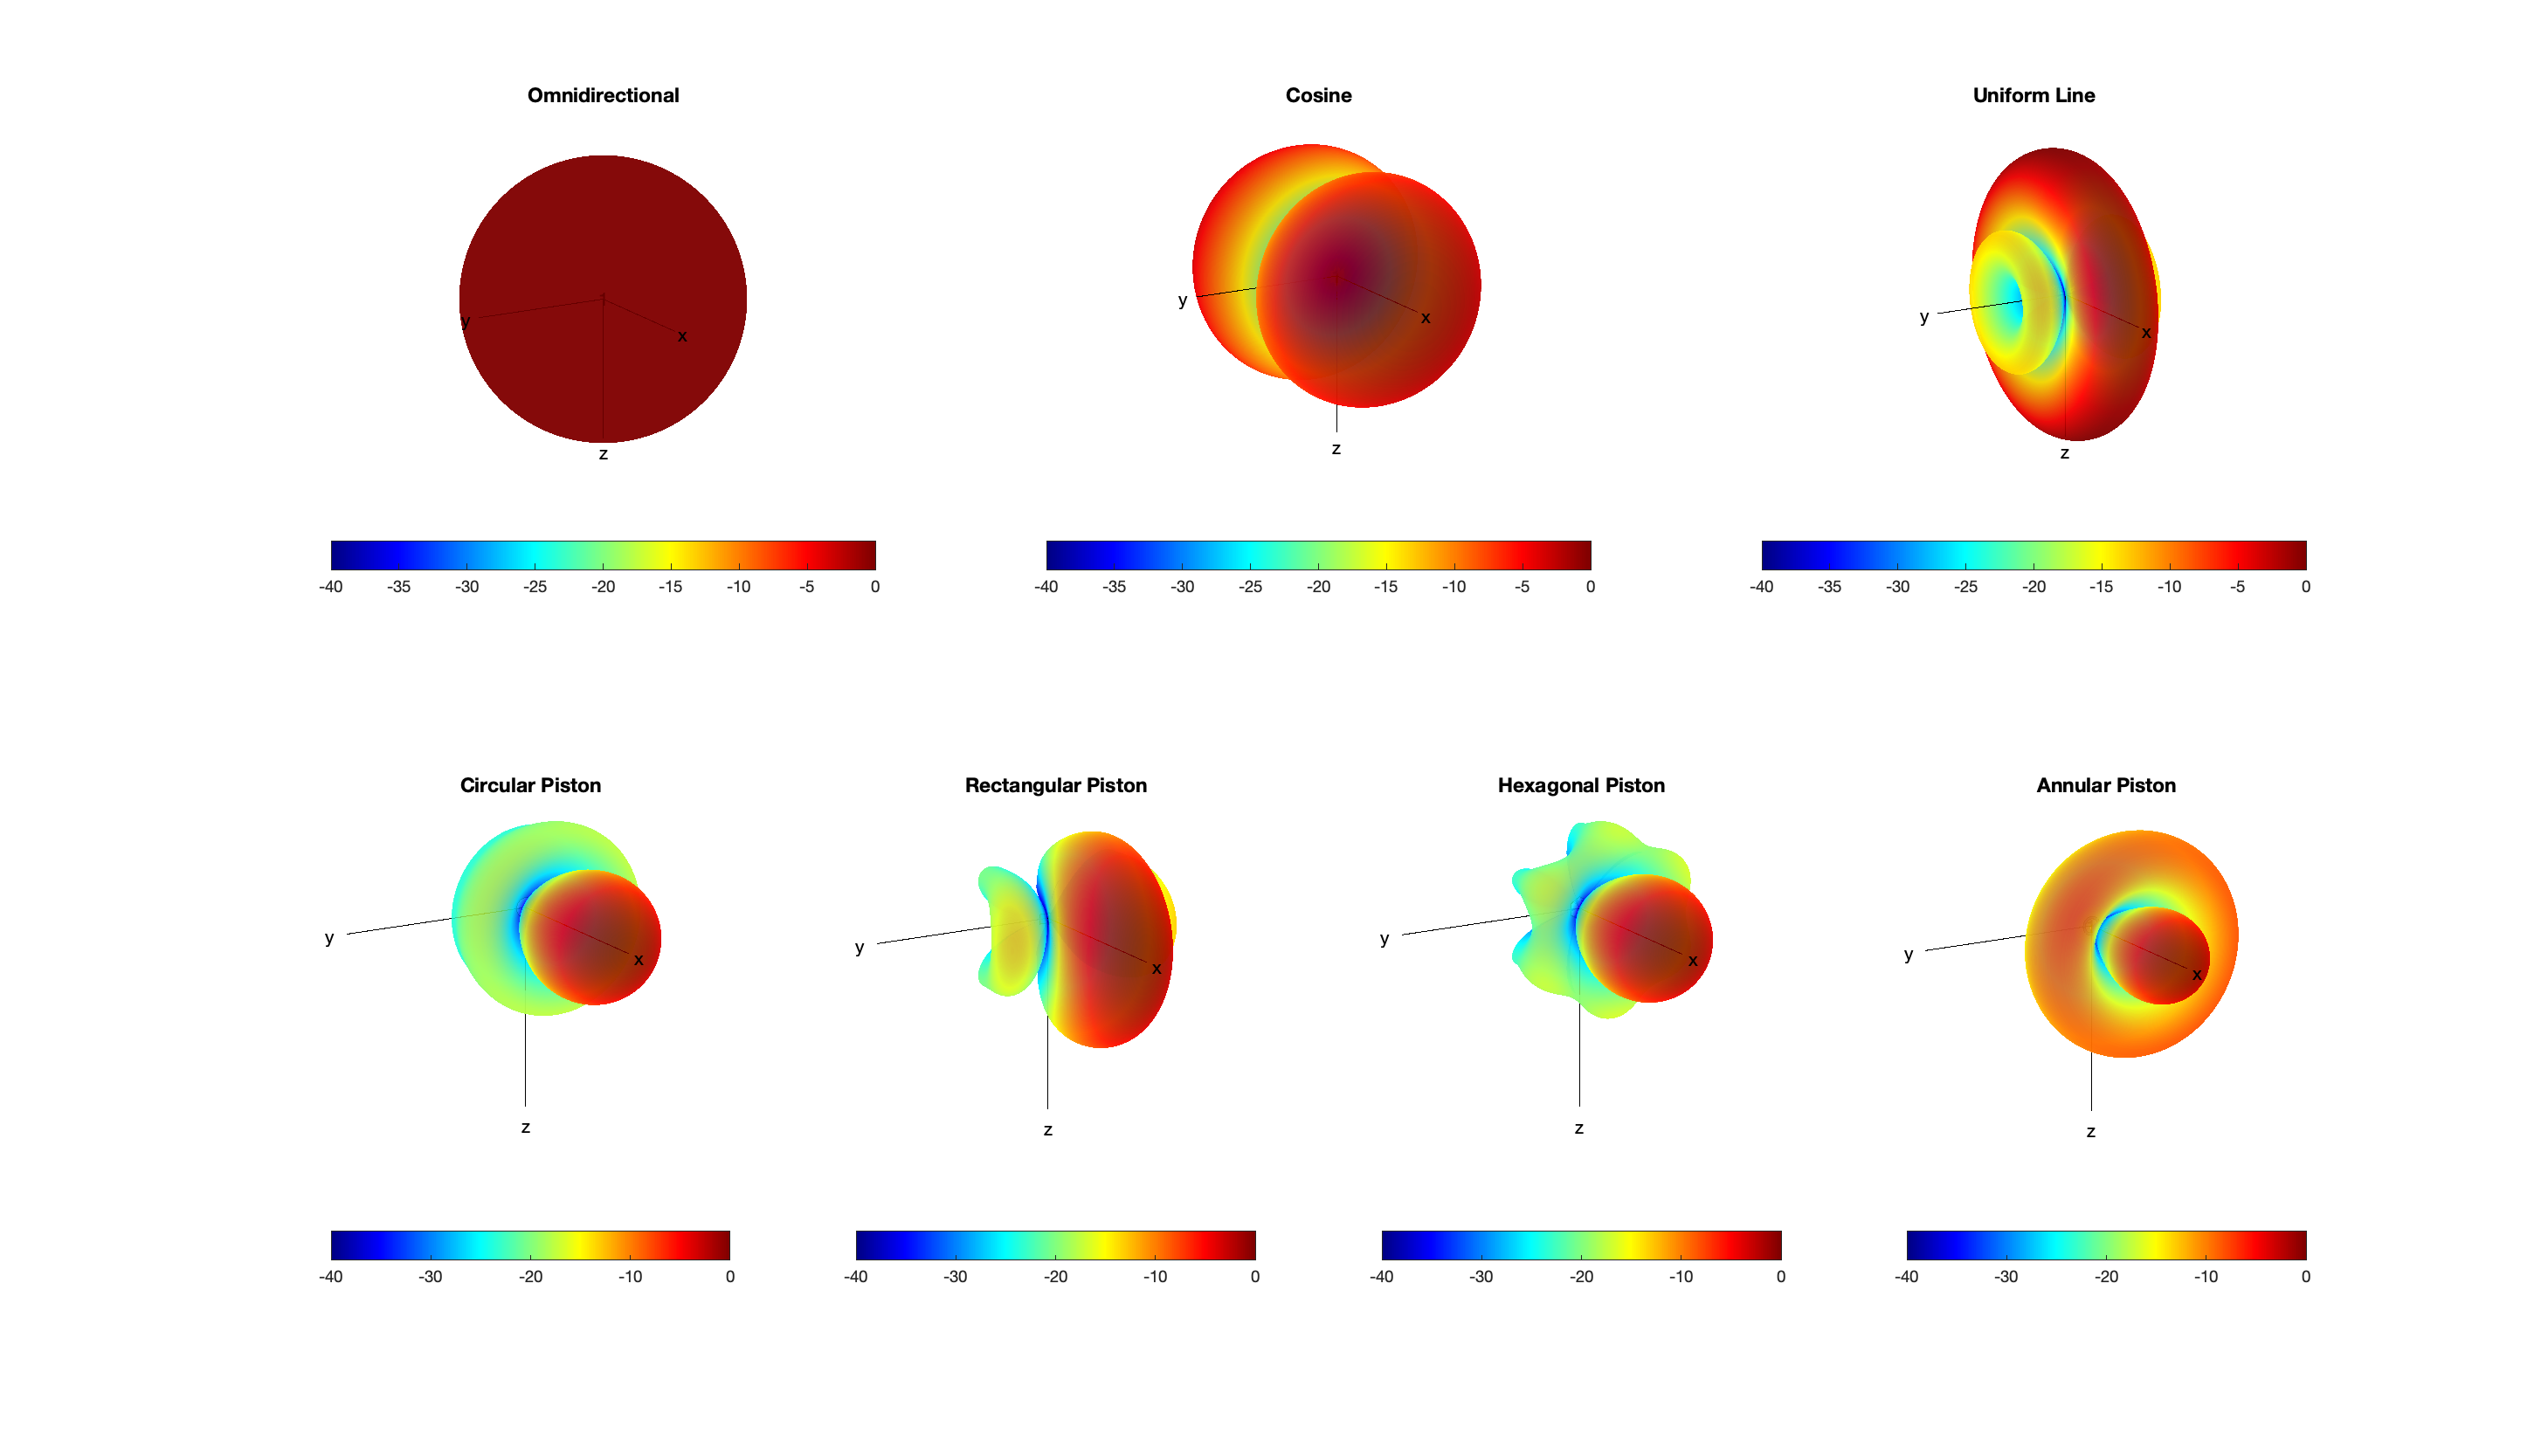
\includegraphics[width=8in]{ElementPatterns}
\caption{\label{fig:ElementPatterns}Element patterns for included element types}
\end{center}
\end{sidewaysfigure}
